\chapter{Theoretischer Hintergrund}
\label{chap:theorie}
Zur Betrachtung von Streuung ist es zweckmäßig, zunächst die benötigten Grundlagen zu definieren, um aus diesen dann die Simulationsansätze sowie die Grundlagen der Rekonstruktion aus Streubildern abzuleiten. Sofern nicht anderweitig gekennzeichnet folgen die Herleitungen Standardwerken~\cite{goodman2005,cowley1995,born1980}.
\section{Skalare Beugungstheorie}
Aus den Maxwell-Gleichungen lässt sich unter der Annahme eines sich im Vergleich zur Wellenlänge $\lambda$ räumlich nur langsam ändernden Mediums die skalare Helmholzgleichung
\begin{equation}
	\label{eq:wellengleichung_r}
	(\Delta+k^2\eta^2)\phi=0
\end{equation}
mit der Wellenzahl $k$
\begin{equation}
	k=\frac{2\pi}{\lambda}
\end{equation} und der komplexen Brechzahl des Mediums $\eta$ für eine elektromagnetische Welle $\phi$ aufstellen. Diese Betrachtung ignoriert den vektoriellen Charakter der Elektrodynamik, insbesondere die Polarisation der Welle wird vernachlässigt. Des Weiteren findet eine Separation der Zeitabhängigkeit statt, sodass nur stationäre Probleme betrachtet werden.

Im Bereich der Röntgenbeugung kann es aufgrund der geringfügigen Abweichungen der Brechzahlen von Medien zur Vakuumbrechzahl ($\eta=1$) hilfreich sein, $\eta$ als
\begin{alignat}{2}
	\label{eq:brechzahl}
	  & \eta   &   & =1-\delta+i\beta=1 + \delta n \\
	\label{eq:approxbrechzahl}
	  & \eta^2 &   & \approx 1 + 2\delta n         
\end{alignat}
darzustellen. Bei dieser Darstellung quantifiziert $\delta$ die Refraktion, $\beta$ die Absorption~\cite{attwood1999}.

Eine für die Betrachtung von Streuvorgängen hilfreiche Form der Wellengleichung lässt sich durch Darstellung mittels einer Greenschen Funktion finden. Hierfür  wird zunächst die Fouriertransformierte der Wellengleichung betrachtet. Mit dem Ortsvektor $\vec{r}=(x,y,z)^T$ im Realraum und $\vec{q}=(q_x,q_y,q_z)^T$ im Frequenzraum lautet diese mit der Näherung \ref{eq:approxbrechzahl} und unter Beachtung des Faltungstheorems (\fref{eq:ft_faltung}) und der Ableitung (\fref{eq:ft_ableitung}) 
\begin{equation}
	\label{eq:wellengleichung_f}
	(-q^2+k^2)\tilde{\phi}=\frac{-2k^2}{{(2\pi)}^{\sfrac{3}{2}}}(\tilde{\delta \eta} \ast \tilde{\phi}) \,.
\end{equation}
Hierbei bezeichnet die Notation $\tilde{f}(q)$ die Fouriertransformierte von $f(r)$. Wird nun die Greensche Funktion  $\tilde{G}$ im Fourierraum als
\begin{equation}
	\tilde{G}=\frac{1}{(2\pi)^{\sfrac{3}{2}}}\frac{2k^2}{q^2-k^2}
\end{equation}
definiert, so lässt sich daraus nicht direkt die Greensche Funktion im Realraum gewinnen, da das Integral der inversen Fouriertransformation von $\tilde{G}$ divergiert. Dieses Problem lässt sich durch Hinzufügen eines infinitesimalen imaginären  $i\epsilon$ (mit $\epsilon\rightarrow 0^+$) zu $k$ im Nenner lösen (\fref{eq:green_ft})~\cite{trigg2006,griffiths2005}.

\begin{align}
	G & =\frac{1}{(2\pi)^{3}}\int_{-\infty}^{\infty} \frac{2k^2}{q^2-(k+i0^+)^2} e^{i\vec{q}\vec{r}}\dif^3 \vec{q}\nonumber \\
	  & = \frac{k^2}{2\pi}\frac{e^{ikr}}{r}
	  \label{eq:green_ft}                                                                     
\end{align}
Die so konstruierte Greensche Funktion lässt sich in den Realraum transformieren, stellt weiterhin eine Greensche Funktion der Wellengleichung dar und wird als \textit{retardierte Greensche Funktion} bezeichnet. Für die Wellengleichung gilt mit ihr somit im Fourier- bzw. im Realraum~\cite{cowley1995,thibault2007}:
\begin{align*}
	\label{eq:wellengleichung_green} \numberthis
	\tilde{\phi} & =\tilde{G}(\tilde{\delta \eta} \ast \tilde{\phi}) \\
	\phi         & ={G}\ast({\delta \eta}  {\phi})                   
\end{align*}
Diese Formulierung erweist sich im Folgenden für die Herleitung der Born-Näherung als hilfreich.
\section{Born-Näherung}
Eine häufige Näherung bei Streuproblemen ist die sogenannte \textit{Born-Näherung}. Sei zunächst mit den in \fref{fig:bornr}  dargestellten Bezeichnungen für die Vektoren das streuende Objekt bei $\vec{r'}$ räumlich um den Koordinatenursprung beschränkt (und somit auch $\delta\eta(\vec{r'})$). Zur Berechnung der Welle am Beobachtungsort $\vec{r}$ wird nun davon ausgegangen, dass gilt $|\vec{r}| \gg |\vec{r'}|$ für alle Punkte an denen $\delta\eta$ von Null verschieden ist, d.h. dass der Beobachtungsabstand groß gegenüber den Ausmaßen des Streuobjektes ist~\cite{griffiths2005}. In diesem Fall gilt die Näherung
\begin{equation}
	\abs{\vec{r}-\vec{r'}} = \sqrt{r^2+r'^2-2\vec{r}\cdot\vec{r'}} \approx r-\frac{\vec{r}}{r}\cdot\vec{r'} \,.
	\label{eq:born_r_approx}
\end{equation}
In \fref{eq:wellengleichung_green} kann nun die Faltung ausgeschrieben und die Greensche Funktion genähert werden (mit $\vec{k}$ als ausgehenden Wellenvektor nach dem Streuvorgang in $\vec{r}$-Richtung):
\begin{equation}
	\phi(\vec{r})=\int G(\vec{r}-\vec{r'})\delta\eta(\vec{r'})\phi(\vec{r}') \dift \vec{r'} 
	\propto \int \frac{e^{ik(r-\vec{k}\vec{r'})}}{r}\delta\eta(\vec{r}')\phi(\vec{r}') \dift \vec{r'} \,.
	\label{eq:born_ort}
\end{equation}
Hierbei wird die Näherung aus \fref{eq:born_r_approx} im Exponenten angewendet. Im Nenner kann aufgrund des geringen (da nur linearen) Einflusses $\abs{\vec{r}-\vec{r'}}\approx r$ genähert werden. Wird nun $\phi$ als Reihe $\phi=\phi_0+\phi_1+\phi_2+..$ mit $\phi_0(\vec{r'})=e^{i\vec{k_0}\vec{r'}}$ als einlaufende ebene Welle dargestellt und ist der Einfluss des Streuobjektes auf die einfallende Welle gering, so lässt sich in \fref{eq:born_ort} $\phi(\vec{r'})\approx\phi_0(\vec{r'})$ im Integral anwenden~\cite{cowley1995}. Dies wird als \textit{Born-Näherung erster Ordnung} bezeichnet. In dieser gilt mit dem Streuvektor $\vec{q}=\vec{k}-\vec{k_0}$ (vgl. \fref{fig:bornq}) und dem Erhalt der Wellenzahl $|\vec{k_0}|=|\vec{k}|$ (elastische Streuung) für die Lösung der Wellengleichung
\begin{equation}
	\label{eq:born}
	\int G(\vec{r}-\vec{r}')\delta\eta(\vec{r}') e^{i\vec{k_0}\vec{r'}}  \dift \vec{r}'
	\approx \frac{e^{ik_0r}}{r}\int \delta\eta(\vec{r}')e^{-i\vec{q}\vec{r}'}\dift \vec{r}'\propto \mathscr{F}[\delta\eta] \,.
\end{equation} 
Dies hat die Form einer Fouriertransformation -- in Näherung ist die gestreute Welle proportional zur dreidimensional fouriertransformierten Abweichung der Brechzahl von der Vakuumbrechzahl.


\begin{figure}
	\centering
	\begin{subfigure}[b]{0.49\textwidth}
		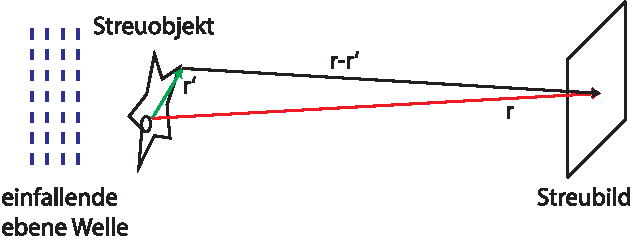
\includegraphics[width=\textwidth]{images/bornr.pdf}
		\caption{Ortsvektoren}
		\label{fig:bornr}
	\end{subfigure}
	\begin{subfigure}[b]{0.49\textwidth}
		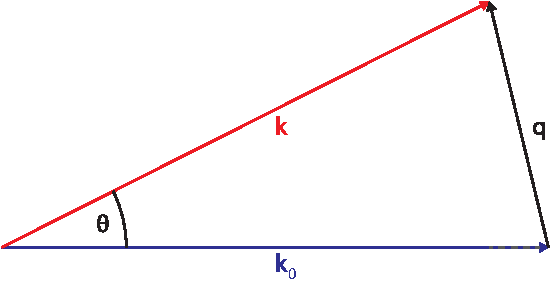
\includegraphics[width=\textwidth]{images/bornq.pdf}
		\caption{Wellen- und Streuvektor}
		\label{fig:bornq}
	\end{subfigure}
	\caption[Geometrie bei Born Näherung]{Skizze zur Bezeichnung der Ortsvektoren (a) sowie
		 der Wellenvektoren und des Streuvektors (b). Das Streuobjekt ist räumlich um den Ursprung beschränkt und liegt bei $\vec{r'}$, die Beobachtung findet bei $\vec{r}$ statt. $\vec{k_{0}}$ und $\vec{k}$ bezeichnen den Wellenvektor der einfallenden bzw. ausfallenden Welle mit dem dazwischenliegenden Winkel $\theta$, $\vec{q}$ bezeichnet den Streuvektor.}
\end{figure} 


\section{Angular-Spectrum Propagation}
Wird eine elektromagnetische Welle $\phi$ durch ihre zweidimensionale Fouriertransformierte $\bar{\phi}$ als
\begin{equation}
	\phi(x,y,z)=\frac{1}{2\pi}\iint_{-\infty}^{\infty}\bar{\phi}(f_x,f_y,z)e^{i(q_xx+q_yy)} \dif q_x \dif q_y
\end{equation}dargestellt und gefordert, dass diese im Vakuum die Wellengleichung \eqref{eq:wellengleichung_r} erfüllt,
so muss $\bar{\phi}$ im Hybridraum ($q_x,q_y$ im Fourierraum, in z-Richtung jedoch im Realraum)
\begin{equation}
	\label{eq:wellengleichung_h}
	\frac{\partial ^2}{\partial z^2}\bar{\phi}(q_x,q_y,z)+ \left(k^2-\left(q_x^2+q_y^2\right)\right)\bar{\phi}(q_x,q_y,z)=0
\end{equation}
erfüllen. Eine Lösung dieser Gleichung ist
\begin{equation}
	\label{eq:angularspectrum}
	\bar{\phi}\left(q_x,q_y,\Delta z\right)=\bar{\phi}(q_x,q_y,0)e^{i\Delta z\sqrt{k^2-(q_x^2+q_y^2)}}\, . 
\end{equation}
Somit lässt sich die Propagation einer Welle im Vakuum als Multiplikation mit einem Exponentialfaktor im Fourierraum beschreiben. Dieses Verfahren wird \textit{Angular-Spectrum} Propagation genannt~\cite{goodman2005}. Die eingehende Welle bei $z=0$ wird hierbei in ebene Wellen, die sich in verschiedene Richtungen ausbreiten (Angular Spectrum) zerlegt und deren Propagation berechnet. Die ausgehende Welle bei $z=\Delta z$ im Realraum, $\phi\left(x,y,\Delta z\right)$, lässt sich aus $\bar{\phi}\left(q_x,q_y,\Delta z\right)$ durch eine inverse Fouriertransformation bestimmen.


\section{Fresnel- und Fraunhofer-Näherung}
\label{chap:fraunhofer}
Wird in \fref{eq:angularspectrum} die Taylor-Näherung 2. Ordnung
\begin{equation}
	\sqrt{k^2-(q_x+q_y)^2}\approx k-\frac{(q_x^2+q_y^2)}{2k}
\end{equation}
durchgeführt (\fref{eq:fresnel_fourier}) und eine zweidimensionale inverse Fouriertransformation angewendet, so erhält man mit dem Faltungstheorem die Fresnel-Näherung im Realraum (\fref{eq:fresnel_real}).

\begin{align}
	\bar{\phi}(x,y, z) &=\bar{\phi}(x,y,0) e^{ik z}e^{\frac{i z}{2k}(q_x^2+q_y^2)} 
	\label{eq:fresnel_fourier}\\
	\xRightarrow{\mathscr{F}^{-1}}  \phi(x,y, z) &=\phi(x,y,0) \ast \left( \frac{e^{ik z}}{i z \lambda } e^{ik\frac{(x^2+y^2)}{2 z}} \right)
	\label{eq:fresnel_real}
\end{align}
In dieser Näherung wird die Ausbreitung der Welle durch die Faltung mit dem sogenannten Fresnel-Propagator ausgedrückt. Wird die Faltung explizit ausgeschrieben, kann der Exponent aufgespalten werden
\begin{align}
\label{eq:fresnel_explizit}
	\phi(x,y, z) & =\frac{e^{ikz}}{iz\lambda}                           
	\int_{-\infty}^\infty 
	\phi(\alpha,\beta,0)
	e^{\frac{ik}{2z}\left(\left(x-\alpha\right)^2+\left(y-\beta\right)^2\right)}
	\dif \alpha \dif \beta \nonumber \\
	             & =\frac{e^{ikz}}{iz\lambda}e^{\frac{ik}{2z}(x^2+y^2)} 
	\int_{-\infty}^\infty 
	\phi(\alpha,\beta,0)
	e^{\frac{ik}{2z}\left(\alpha^2+\beta^2\right)}
	e^{\frac{-ik}{ z}\left(x\alpha+y\beta\right)}
	\dif \alpha \dif \beta \,.
\end{align}
Verschwindet nun die eingehende Welle $\phi(x,y,z=0)$ außerhalb eines Bereiches $S=[-X,X]\times[-Y,Y]$ und gilt 
\begin{equation}
	\forall \alpha,\beta \in S:	z\gg \frac{k}{2}\left(\alpha^2+\beta^2\right) \, , 
\end{equation}
d.h. sind die Ausmaße des Bereiches, auf dem die Welle nicht verschwindet klein gegenüber dem Beobachtungsabstand, so gilt
\begin{equation}
	e^{\frac{ik}{2z}\left(\alpha^2+\beta^2\right)}\approx 1 \,.
\end{equation}
So lässt sich \fref{eq:fresnel_explizit} als Fouriertransformation der Eingangswelle ausgewertet bei $f_{x,y}=\tfrac{k}{z}(x,y)$ und multipliziert mit einem in $x,y$-Richtung reinem Phasenterm interpretieren (\fref{eq:fraunhofer}). Diese Näherung wird als Fraunhofer-Näherung bezeichnet und lässt sich zur Berechnung des Fernfeldes einer elektromagnetischen Welle verwenden.

\begin{equation}
\label{eq:fraunhofer}
	\phi(x,y,z)=\frac{e^{ik(z+\frac{x^2+y^2}{2z})}}{iz\lambda}\mathscr{F}\left[\phi(x,y,0)\right](f_x=\tfrac{kx}{z},f_y=\tfrac{kx}{z})
\end{equation}


